\documentclass{article}

\usepackage{times}
\usepackage{graphicx}
\usepackage{subfigure}
\usepackage{natbib}
\usepackage{algorithm}
\usepackage{algorithmic}
\usepackage{lipsum}
\usepackage{todonotes}
\usepackage{amssymb}

\usepackage{hyperref}
\usepackage{tikz}
\usetikzlibrary{bayesnet}

\usepackage[accepted]{icml2017}
\icmltitlerunning{CS 281 Final Project Template}

\begin{document}

\twocolumn[
\icmltitle{Automated, Scalable Signal Region Identification with Applications to the ATLAS W$^{\pm}$W$^{\pm}$W$^{\mp}$ Analysis}
\begin{icmlauthorlist}
  \icmlauthor{Nicol\`o Foppiani}{}
  \icmlauthor{Jonah Philion}{}
  \icmlauthor{Baojia Tong}{}
\end{icmlauthorlist}

\vskip 0.3in
]

\begin{abstract}

The aim of this work is to use machine learning to maximize the capability of particle physics experiments to discover new phenomena.

In a typical particle physics experiment, detector data from trillions of particle collisions are recorded. During each collision, various physics processes randomly occur, each with some probability. The time steps are data points, and the particles measured by the detector are the features of the data points.

To discover a new phenomenon, physics processes are divided into two categories: the known and already discovered \textit{background}, and a new, undiscovered \textit{signal}. All events are assumed to be generated from either a background or signal process. Discovery is claimed when the distribution of observed data points is incompatible with the background expectation.

Our approach is to use machine learning techniques to identify the \textit{signal region} in the multidimensional space of detector features. The signal region is the volume of parameter space with the largest significance of signal with respect to the background. Instead of enforcing that the signal region be rectangular as is traditionally done in particle physics experiments, we leverage the output of contemporary classification algorithms to identify a more flexible signal region.

The approach is tested on simulations of W$^{\pm}$W$^{\pm}$W$^{\mp}$ production in the presence of a WZ background at the ATLAS experiment. The statistical models improve expected significance over rectangular cuts by 43\%. Physics-driven interpretations of the classifiers are discussed. Code for this paper is available \href{https://github.com/tongbaojia/cs281_mlphys}{here}

\end{abstract}


%%%%%%%%%%%%%%
\section{Introduction}
\label{sec:introduction}
%What is the problem of interest and what (high-level) are the current best methods for solving it? -- 
%How do you plan to improve/understand/modify this or related methods? -- 
%Preview your research process, list the contributions you made, and summarize your experimental findings. -- 
Given a dataset from a particle collider, particle physicists would like to determine the phenomena that generated the dataset. A collision  - known as an \textit{event} - is a data-point in the dataset. Events are assumed to be independent of each other because they represent distinct collisions. Each event has a label identifying the physical process that generated the event and features measured by the detectors. In a real dataset from the ATLAS detector, the labels must be inferred.

Synthetic datasets also come equipped with a set of weights. Weights are computed in simulation such that the synthetic dataset has the same proportion of signal and background events as real datasets collected by the experiment. All histograms, ROC curves, and significance are computed using these weights instead of raw counts.

% The discovery of a new physical process is extremely important in particle physics: the new process of interest, which the experiment aims to discover, is called signal, whereas the other physical processes, that can fake the signal, are collectively called background.  
Typically, in a real dataset collected by the experiment, a mixture of background and signal data-points are collected. The number of signal and background data-points follow the Poisson distribution. If the number of expected signal events is greater than the statistical fluctuations of the background, the signal process is verified. This is formally quantified using the \textit{significance}, which is defined in terms of a statistical test. 

The problem is to identify the region in the feature space with the largest possible significance. In particle physics, identification is often performed by choosing hyper-rectangles in the feature space. The choice of the hyper-rectangle is often guided by the physical understanding of the processes and of the meaning of the features that are collected.
However, this procedure cannot a efficiently select a non-linear region in the feature space. It is neither automated nor scalable. This work provides a procedure based on machine learning to select the optimal non-linear signal region to compute the significance.
The problem has been factored into two steps. In the first step, we use machine learning to determine a representation of the parameter space which separates the signal events from the background events. In the second step, the region with the highest significance is built with the points of higher signal to background ratio.

This method has been tested on a dataset provided by the ATLAS experiment, affiliated with the W$^{\pm}$W$^{\pm}$W$^{\mp}$ analysis. For this analysis a previous study using a hyper-rectangular signal region is present. We define the result from that paper to be the baseline for this project. Three classification algorithms have been studied, namely logistic regression (one-layer neural network), deep neural networks, and boosted decision trees. The result of our algorithm is compared with the baseline, both in terms of classifier performance and in terms of significance, showing a good improvement with respect to the baseline. 

The power of these adaptive basis features are evaluated against features which the Standard Model suggests should be strong discriminators for WWW production analysis. 

% This study tries to optimize the region in the feature space that gives the greatest significance for the W$^{\pm}$W$^{\pm}$W$^{\mp}$ process.
% \paragraph{}
% Previously this study were treated with hyper-rectangles in the feature space. The choice of the hyper-rectangle is often guided by the physical understanding of the processes and of the meaning of the features that are collected.
% \paragraph{}
% In this work, machine learning techniques are used to identify the signal region. The goal is to find the best classification algorithm which distinguish signal and background. The output of a classifier is then used to identify regions with large fractions of signal events with respect to the background events. 
% \paragraph{}
% Three algorithms have been developed: logistic regression, deep neural networks and boosted decision trees from XGBoost. The performance is tested in terms of the significance. The algorithm has been tested on the ATLAS W$^{\pm}$W$^{\pm}$W$^{\mp}$ analysis. The feature space is also evaluated from machine learning perspective, and the performance is further evaluated and interpreted in terms of physics-driven variables. The algorithms show great improvements with respect to the baseline for this analysis, revealing the power of machine learning, yet the interpretation reveals the limitations and the importance of feature engineering.


%%%%%%%%%%%%%%
\section{Background}
\label{sec:backgroiund}
%What information does a non-expert need to know about the problem domain? -- 
%What data exists for this problem? -- 
%What are the challenges/opportunities inherent to the data? (High dimensional, sparse, missing data, noise, structure, discrete/continuous, etc?) -- 

In particle physics, discovering a new process is an important step. A discovery is performed on a statistical basis, in terms of a statistical test. This means to understand if the number of expected signal data-points is compatible with the statistical fluctuations of the number of expected background events. The output of the statistical test is called \textit{significance}: this is a well established metric in physics, and its optimization represents the final goal of this work. A detailed description about significance and theoretical way to optimize is given in reference \cite{Punzi_significance}. However, for the purpose of this study, a summary of the required knowledge is following.
Given a certain region in the feature space space delimited by a non-linear contour, it is possible to estimate the number of expected events belonging to that region which are labeled as signal ($S$) and the number of events labeled as background ($B$). The problem is to understand if the signal is significant, or in other words, if the signal is likely to be a statistical fluctuation of the background. To quantify this significance, usually a statistical test is performed. In the hypothesis in which there is no signal, the number of events in the selected region is drawn from a Poisson with mean $B$.
\[ n \sim Pois(\mu = B) \]

In case that B is large, so that the distribution of n can be approximated with a normal distribution:
\[ n \sim \mathcal{N}(\mu = B, \sigma^2 = B) \]
Now it is possible to quantify the expected significance. Since $n$ is drawn from this distribution 
\[z = \frac{n-B}{\sqrt{B}} \sim \mathcal{N}(0, 1)\]
If the signal is present, we expect $n = S + B$, thus, 
\[z = \frac{S}{\sqrt{B}}.\]
If $z \simeq 0$, the expected number of events of signal $S$ is compatible to be a statistical fluctuation of the background $B$. On the contrary, if $z$ is large, it is unlikely for the background to fake the signal: thus the experiment will be able to observe and discover the signal process. Usually in particle physics a significance of at least 3 is required for making an observation, and $z > 5$ to claim a discovery. 

It is worth noting the importance of the p-value of the distribution of the $z$ variable. In fact, it is possible to compute the significance even in the case of small number of background expected events $B$ \cite{cowan_stat}, and the result can be translate into a $z$ variable, equivalent in meaning to the one before, although not Gaussian distributed:
\[ z = \sqrt{2 \left( (S+B) \log \left(1 + \frac{S}{B} \right) - s \right)}\]
This equation is derived from the Poisson PDF and makes no assumption of large $n$. This forms our final evaluation metric.

Generally speaking, particle physics experiments collect big dataset (several millions of data-points) and produce even larger amount of synthetic data.
These dataset contains several simple features, that corresponds to the properties of all the particles produced during a collision, which are measured in the detector. These feature can be discrete and continuous. The number of particles produced in a collision can be very large, and usually only the most important ones are considered. Additionally, the large amount of simple features gives the possibility to build constructed features, usually physically driven. 
The main challenge in using these datasets to observe and discover new physical processes is represented by the small signal to background ratio. Typical signal of interests are very tiny, and the background can be even $10^5$ larger.

In this specific project, a synthetic dataset from the ATLAS experiment has been used. It is related to the analysis for the observation of the $W^{\pm}W^{\pm}W^{\mp}$ process.
The ATLAS detector is one of the two main experiments at the Large Hadron Collider (LHC), currently operating at CERN (Geneva, Switzerland).
The ATLAS collaboration has previously published an analysis \cite{Aaboud:2016ftt} on this process in 2016.
This study was done in the traditional way of selecting a signal region using an hyper-rectangular region. This optimization led to a remarkable result, yet not enough to observe the process of interest. An important point of this previous work was the splitting of the data-points into three different categories, labeled by the \textit{SF0S} variable, which is chosen by a physics insight on the process of interest. In this work it has been decided to keep this splitting, in order to make an easier comparison with respect to the previous work.

% \paragraph{}
% The search project is to measure the triboson production for the first time using the ATLAS detector, one of the two main experiments at the Large Hadron Collider(LHC). Specifically, the signal process under study is the following: $pp \rightarrow W^{\pm}W^{\pm}W^{\mp}$. The $W$ bosons are not detected directly as they decay immediately into a lepton and a neutrino. The lepton, in this case an electron ($e$) or a Muon ($\mu$), can be measured by the ATLAS detector. The neutrino escapes the detector without interaction, but can be inferred using conservation of momentum. The final state, while requiring three leptons, is further split into three orthogonal states based on the charge and flavor composition of the leptons, as Same Flavor Opposite Sign (SFOS) pairs. The available SFOS states are discrete due to the conservation of charge, as 0, 1 and 2. This is important as the background composition varies drastically in each different states.
% \paragraph{}
% This project probes the so-called ''quartic coupling'': a quantity which is predicted by the current theory of the fundamental interactions, called Standard Model(SM) to be small. This process hasn't been observed yet, however, if the current theory is not correct, it would be expected an important difference between the measured value of this quantity and the prediction. This could be an insight toward some new physics process, not yet discovered, which could completely change our understanding of fundamental nature. With the higher center of mass energy of the collisions and the newer and larger data-sets collected during the last few years, the probability for this process to happen should be large enough in order to produce several such events.
% \paragraph{}
% However, there exists a great variety of well known processes which mimic the signal and which therefore are called background. Different other electroweak processes ($W^{\pm}W^{\mp}$, $ZZ$, $W^{\pm}Z$) have about $O(10^3)$ times higher rate and can also generate signatures that are similar to the signal. Other SM processes like $t\bar{t}$ have about $O(10^5)$ times higher rate, and can generate decay products that fake the signal signatures in the detector.
% \paragraph{}
% The ATLAS experiment has done a search \cite{Aaboud:2016ftt} on this process in 2016. The search used real collision events, and Monte Carlo(MC) events, where the signal and backgrounds are modeled at generator level, and further fully simulated to describe multi-particle interactions and detector effects.  In 2017, the LHC is delivering collision events at higher center of mass energy, and increases the discovery potential. The current data is not accessible yet, however, the MC events are available, which form the input for this study. These MC events are further processed and selected, to make the signal and background have at least the same number of basis variables.
% \paragraph{}
% The main challenge for discovery is the small signal yield compared with the enormous and complicated background. The way to distinguish between the signal and the background is to characterize the events with multiple features which can be used to classify the events in signal and background. These features are based from detector measurements, but could be recombined into higher level observable. Therefore, one of the major challenge is the feature engineering, and then the corresponding high dimension feature space. This also bring great improvement potentials for the machine learning algorithms.

%%%%%%%%%%%%%%
\section{Related Work}
\label{sec:rw}
%What 3-5 papers have been published in this space? -- 
%How do these differ from your approach? -- 
%What data or methodologies do each of these works use? -- 
%How do you plan to compare to these methods? -- 

% \paragraph{}
Several theoretical work has been written about the significance and its optimization, yet most studies with experimental data relies on the technique which identifies the signal region with an hyper-rectangular border. This is obtained by looking at the distribution of each feature and by the deciding, feature by feature, which region contains more signal. 
The approach discussed in this work differs from the previous one because it allows the signal region to be non linear, and it construct it with machine learning techniques, in terms of the output of a classifier algorithm.

For the specific dataset which has been used for this work, the paper relative to the previous analysis is available \cite{Aaboud:2016ftt}. It is based on the previous approach with a manual optimization, but leading with a remarkable result. The result of this previous work, which has been reproduced for the sake of comparison, makes up the baseline for this project.

The two methods will be compared into two steps, which resemble the way the problem has been decomposed to.
First of all, the classification algorithms are compared with the baseline in terms of true and false positive rates. Then the result will be further compared in terms of the significance of the signal.

%%%%%%%%%%%%%%
\section{Model}
\label{sec:model}
%What is the formal definition of your problem? -- 
%What is the precise mathematical model you are using to represent it? In almost all cases this will use the probabilistic language from class, e.g. --
% What are the parameters or latent variables of this model that you plan on estimating or inferring? Be explicit. How many are there? Which are you assuming are given? How do these relate to the original problem description? 

The definition of the problem is to define the region of the feature space in which the significance, $z$, is maximum. This is achieved by dividing the problem into two steps: the first one requires the introduction of a classification problem to separate signal and background. \\
To reach this goal the problem is modeled as a logistic regression: we model the probability of the labels $y$ (signal or background) given the features $x$.
\begin{equation}
\label{eqn:y_distribution}
    y \sim Ber(f(x)) 
\end{equation}
where $f(x)$ is any function $\mathbb{R}^n \rightarrow \left[0,1 \right]$.


% \begin{figure}
%   \centering
%   \missingfigure[figheight=8cm]{}
%   \caption{\label{fig:diagram} Directed graphical model describing the problem}
% \end{figure}

\begin{figure}[!h]
  \centering
  \begin{tikzpicture}
  %Define nodes
  \node[latent]                               (x) {$\mathbf{x}$};
  \node[latent, above=of y]  (y) {$y$};
  \node[latent, right=2cm of x]            (w) {$w$};
  % Connect the nodes
  \edge {y} {x} ; %
  \edge {w} {x} ;
  % Plates
  \plate {yx} {(x)(y)} {$N$} ;
  \end{tikzpicture}
  \caption{\label{fig:diagram} Directed graphical model for the logistic regression: $\mathbf{x}$ represents the vector of features, $y$ is the class label, and $w$ represents the parameters of the architecture.}
\end{figure}

% \paragraph{}
The classifier is used to predict the probability for a certain event to be signal for each point of the feature space. The region which maximize the significance is then chosen optimizing a selection on this variable. It is expected that a region with abundant signal with respect to the background is more likely to deliver a large significance.

% \paragraph{}
These models have several parameters, depending of the chosen architecture, that are estimated with a supervised learning approach. 

% \paragraph{}
Three different architectures have been studied.
\begin{itemize}
    \item Simple logistic regression (one layer neural network): this architecture has one weight for each input feature plus a collective bias.
    \item Deep neural networks
    \item Boosted Decision trees: the XGBoost library \cite{xgboost} has been used in this context.
\end{itemize}

The parameters of the neural networks are weights and biases for each neuron. For the case of decision trees, the parameters are the values of the cuts on the various variables in each step of the tree.

%%%%%%%%%%%%%%
\section{Training}
%How do you plan on training your parameters / inferring the states of your latent variables (MLE / MAP / Backprop / VI / EM / BP / ...)
%What are the assumptions implicit in this technique? Is it an approximation or exact? If it is an approximation what bound does it optimize?
% What is the explicit method / algorithm that you derive for learning these parameters?
% \paragraph{}
The training is performed in a supervised way, using MLE inference. Assuming equation \ref{eqn:y_distribution}, the loss function is the well known binary cross-entropy:
\[ L = \sum_i w_i \left( y_i \log(f(x_i)) + (1 - y_i) \log(1 - f(x_i)) \right) \]
The training is done using backpropagation through the network nodes for the two cases of logistic regression and deep neural network. For the boosted decision tree, it has been decided to rely on the black-box algorithm of XGBoost.


%%%%%%%%%%%%%%
\section{Methods}
% What are the exact details of the data-set that you used? (Number of data points / standard or non-standard / synthetic or real / exact form of the data) --
% What are the exact details of the features you computed? -- 
% How did you train or run inference? (Optimization method / hyperparameter settings / amount of time ran / what did you implement versus borrow / how were baselines computed).
% What are the exact details of the metric used? 

% \paragraph{}
The dataset consists of 570k events of synthetic data, which are simulated with a Monte Carlo technique using the ATLAS software. About one third of the data-points has label \textit{signal}, whereas the rest is labeled as \textit{background}. The dataset has been divided in training, validation, and test sets, containing about 70\%, 15\%, and 15\% of the data-points, respectively.
% \paragraph{}
The dataset is pre-processed in order to transform all the discrete features in one-hot variables and to standardize all the continuous variables, by subtracting the mean and rescaling to unitary variance.
% \paragraph{}
The significance is further evaluated in the three independent SFOS regions. It is noteworthy that, if computing the significance selecting as region the whole feature space, the results would be 0.46, no significant at all.
% \paragraph{}
% There are 21 features for each data-point, plus the label and the weight. For each of the three leptons, its $p_T$, $\eta$, $\phi$, mass, charge and electron or muon is saved as a feature, which forms 18 features. The other 9 features are the leading jet $p_T$, $\eta$, $\phi$, mass, inferred missing transverse momentum and direction. On top of these, 24 additional higher level features have been computed from three possible two lepton pairs and the sum of all three leptons. These are physical motivated quantities, which are in general non-linearly transformed from the previous features. This computation should improve the performance of the adaptive basis in the classification, and part of the learning test is to see if the ML methods could recover some of these higher level features, in case those are not directly in the training set.

There are 21 \textit{simple features} for each data-point, plus the label and the weight.
These features are related to the quantities measured experimentally related to the various particles produced in each event.
On top of these, 24 additional \textit{constructed features} have been computed. These features are computed by combining the simple features in physically meaningful variables, that are known to carry information about the process. This computation should improve the performance of the adaptive basis in the classification. Moreover, a dedicated discussion to understand if the ML methods could recover some of these higher level features, in case those are not directly in the training set, has been carried out in the following. In the next, the words \textit{simple} and \textit{constructed} will be used to refer and distinguish the two different kind of features.

% \paragraph{}
The training is optimized differently for the different architectures. In the case of the neural networks (one layer and three layers) the PyTorch library has been used.
The training is performed in batches of 200 data-points, run for 10 epochs. At each epoch the dataset is reshuffled. The weights and the biases are initialized randomly. The optimization is performed with Adam \cite{adam}, set with learning rate = $10^{-3}$ and weight-decay = $10^{-5}$. There parameters are found to be optimal for a reliable and fast convergence.
Concerning the boosted decision tree, the training parameters are chosen to be learning rate of 0.1, number of estimators of 100, maximum depth of 5, minimum child weight of 1.
Both the training of the neural network and of the boosted decision tree last for about 5-10 minutes on a laptop with a Intel Core i5 cpu.

% \paragraph{}
% In order to make a proper comparison with the baseline, the previous cut-based-analysis is reproduced and the significance is compared with the ML outputs.

%%%%%%%%%%%%%%
\section{Results}
%What were the results comparing previous work / baseline systems / your systems on the main task? --
%What were the secondary results comparing the variants of your system? --
%This section should be fact based and relatively dry. What happened, what was significant? --

% \paragraph{}
The first important result is the improvement in the performance with respect to the baseline. The various classifiers are compared by looking at the ROC curves, and quantifying the area underlying it, as shown in figure \ref{fig:roc}.

\begin{figure}[!h]
  \centering
  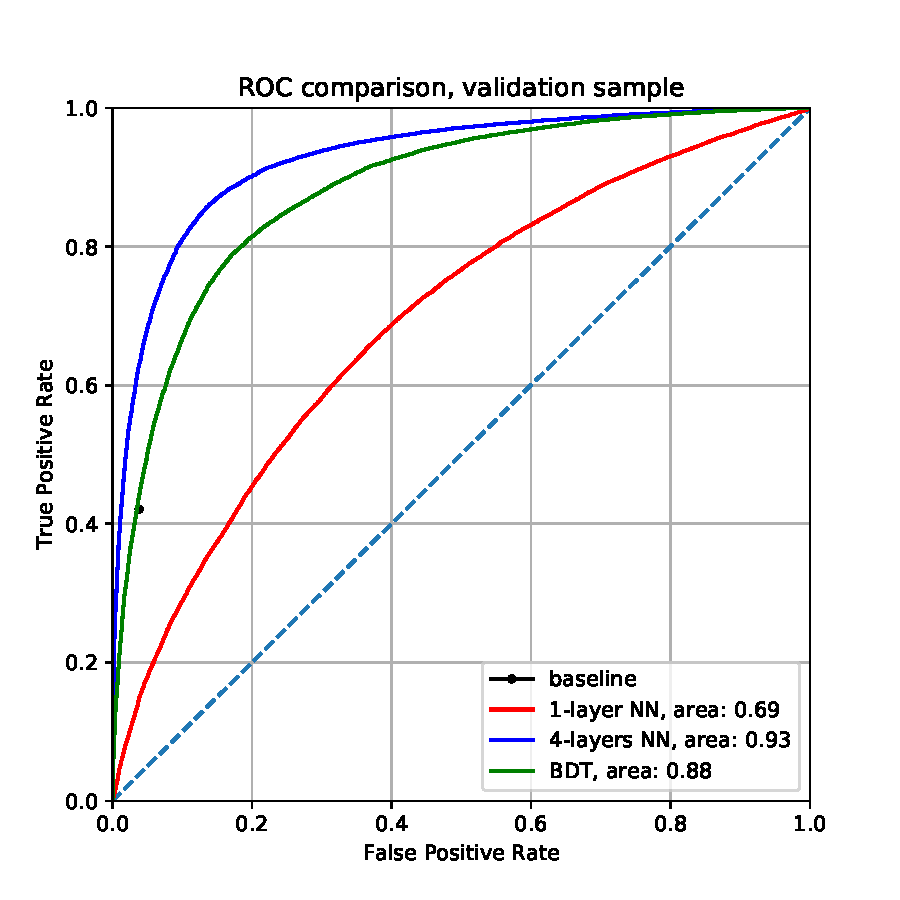
\includegraphics[width=\columnwidth]{roc_curves.pdf}
  \caption{ROC curves on the validation sample. The x-axis is the false positive rate, the y-axis is the true positive rate. The baseline is shown as a dot; the logistic regression is shown as the red curve, the BDT is shown as the green curve and the Neutral Network is shown as the blue curve.}
  \label{fig:roc}
\end{figure}

% \paragraph{}
This plot shows that there is a significant difference between the various architectures. The XGBoost classifier (green line) works much better than the one-layer neural network (red line). The 4-layers neural network (blue line) works better than XGBoost, showing a very good improvement with tuning the parameters. The baseline (black dot) compares well with the two most powerful architectures, although the machine learning algorithms work better than the baseline.

% \paragraph{}
The second important result is the improvement with respect of the baseline in terms of the significance. The plot \ref{fig:significance} shows the result, for the three different physical regions determined by the value of $SFOS$. This result is computed using the test set and the deep neural network architecture.

\begin{figure}[!h]
  \centering
  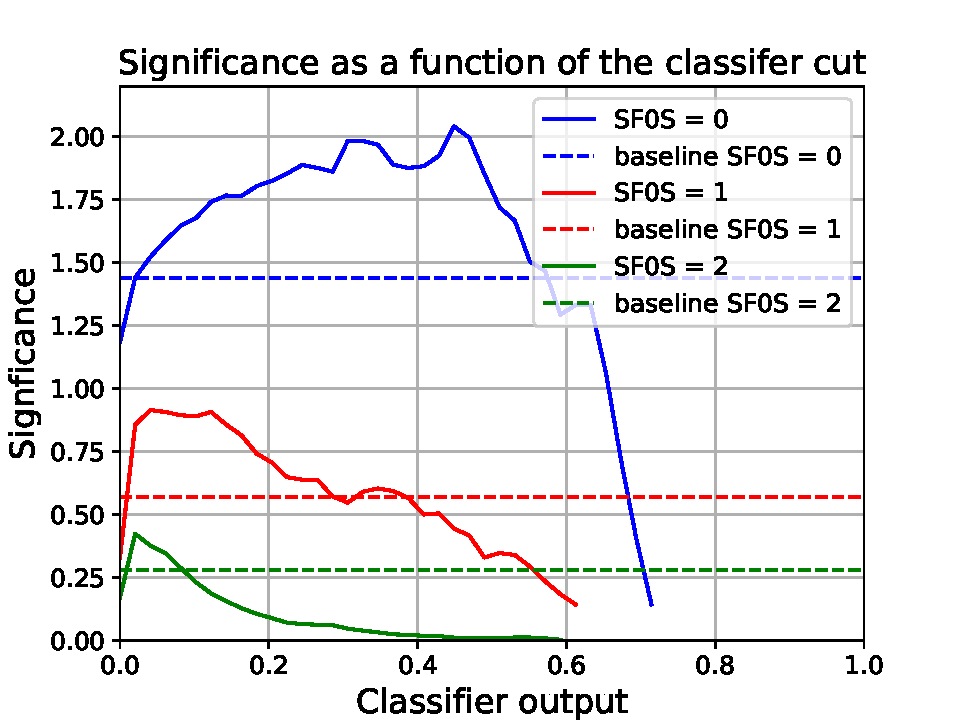
\includegraphics[width=\columnwidth]{significance_with_cuts.pdf}
  \caption{Significance as a function of the region determined by the selection on the classifier cut. The study is produced for the three different regions determined by the value of the variable \textit{SF0S}.}
  \label{fig:significance}
\end{figure}

% \paragraph{}
For each value of $SFOS$, an optimization study of the significance versus the classifier output is performed. Defining the classifier output as $\theta$, the significance is computed considering all the event with $\theta \leq \bar{\theta}$ for different values of $\bar{\theta}$ between 0 and 1. Then the optimal $\bar{\theta}$ is computed. This requirement defines a non-linear boundary in the feature space, in which the significance is computed. In all the three regions the baseline is surpassed by about 25/30\%, showing a remarkable improvement with respect to the previous technique. The result is summarized in table \ref{tab:results}.

\begin{table}[!h]
\centering
    \begin{tabular}{l|l|l|l|l}
    Method              & SF0S=0 & SF0S=1 & SF0S=2 & combined \\
    \hline
    Baseline            & 1.44   & 0.57   & 0.28   & 1.57     \\
    DNN                 & 2.05   & 0.85   & 0.39   & 2.25     \\
    \end{tabular}
\caption{Summary of the result of the significance optimization with respect to the baseline. The result is shown for the three different regions identified by the variable \textit{SF0S}. The column combined indicates the significance obtained by combining the three different regions. The improvement of about 43\% is a remarkable result of this work.}
\label{tab:results}
\end{table}

% \begin{table}
%   \centering
%   \missingfigure[figheight=5cm]{}
%   \caption{Secondary table or figure in results section.}
%   \label{fig:mainres}
% \end{table}


%%%%%%%%%%%%%%
\section{Discussion}
% What conclusions can you draw from the results section?
% Is there further analysis you can do into the results of the system? Here is a good place to include visualizations, graphs, qualitative analysis of your results.
% What questions remain open? What did you think might work, but did not?

% \paragraph{}
The machine learning method shows improvements relative to the baseline analysis, as expected. It is therefore important to further understand the output of the classification algorithm.

% \paragraph{}
For this purpose, the XGBoost algorithm has been chosen, since it has been found easier to investigate the output of the decision tree with respect to the neural network, and because of the simple built-in functions of the library.
Figure  ~\ref{fig:feature_ranking} shows the ranking of the input features. The features are ranked by XGBoost by summing up how many times each feature is split on. It is worth noting that most of the high-ranking features are actually part of the constructed features, which has the result of the feature engineering performed on top of the simple ones.

\begin{figure}[!h]
  \label{fig:feature_ranking}
  \centering
  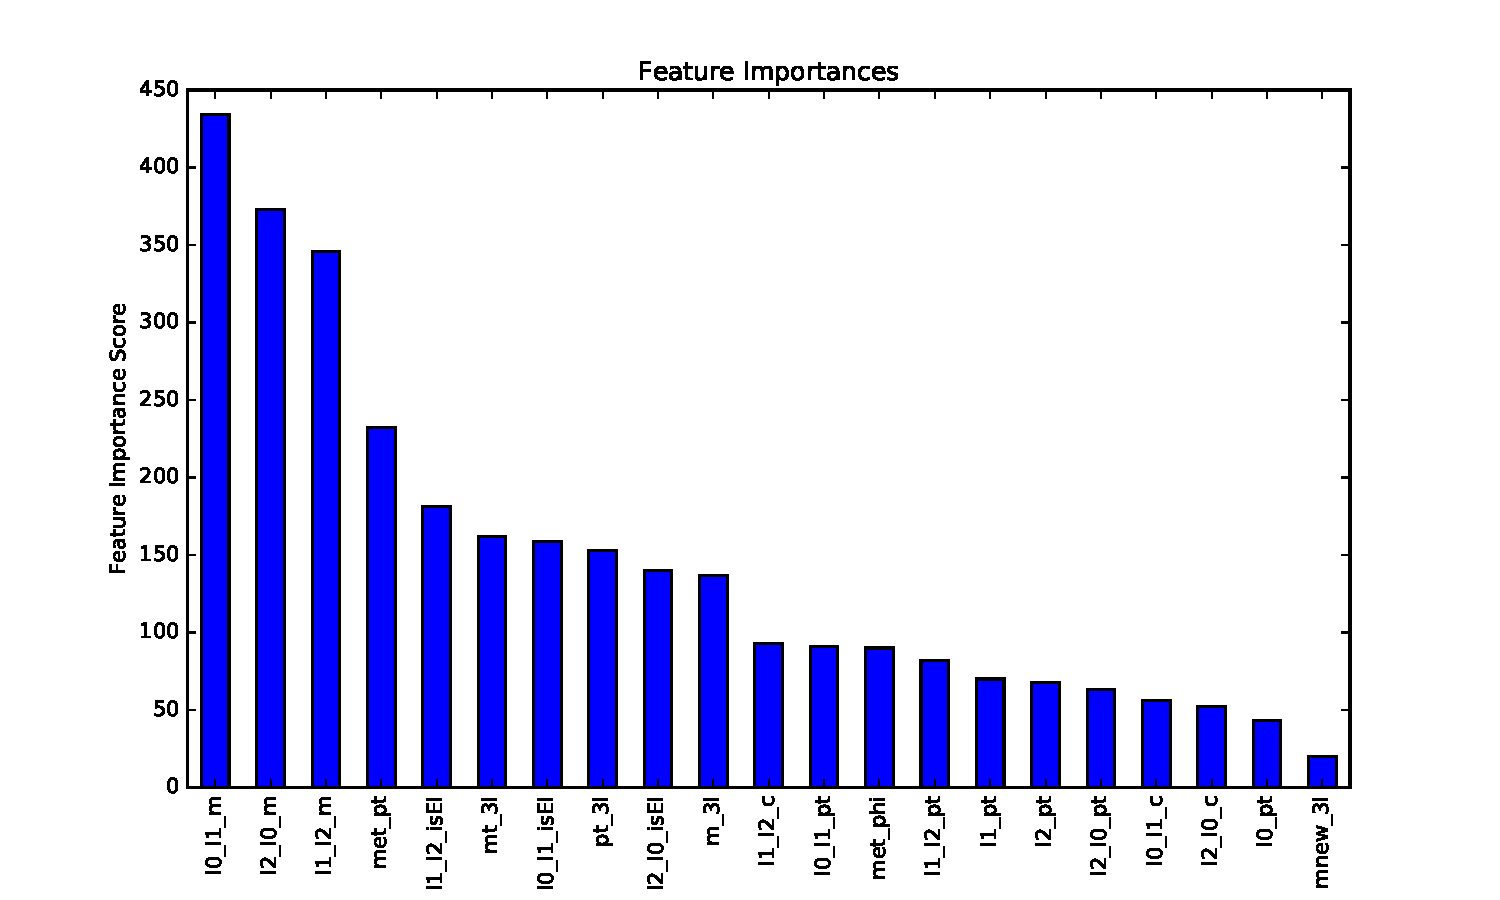
\includegraphics[width=\columnwidth]{feature_ranking_highlevel.pdf}
  \caption{Ranking of features performed with XGBoost.}
\end{figure}

% \paragraph{}
To further evaluate the high-ranking features, those constructed features are removed from the training pool, indicated with $l_{a} l_{b}$ labels. A separate XGBoost classifier is trained using only the simple features. In principle, if the XGBoost adaptive basis recovers all the non-linear transformation which has been done to produce the constructed features, the test output should be similar in the two cases. 
% The test ROC area is shown in Figure ~\ref{fig:roc_curve_lowlevel}. 
However, the performance results to be worse than the baseline XGBoost shown before. Specifically, the area under the ROC curve results to be 0.78 instead of 0.88, which is a significant difference.
% \begin{figure}[!h]
%   \label{fig:roc_curve_lowlevel}
%   \centering
%   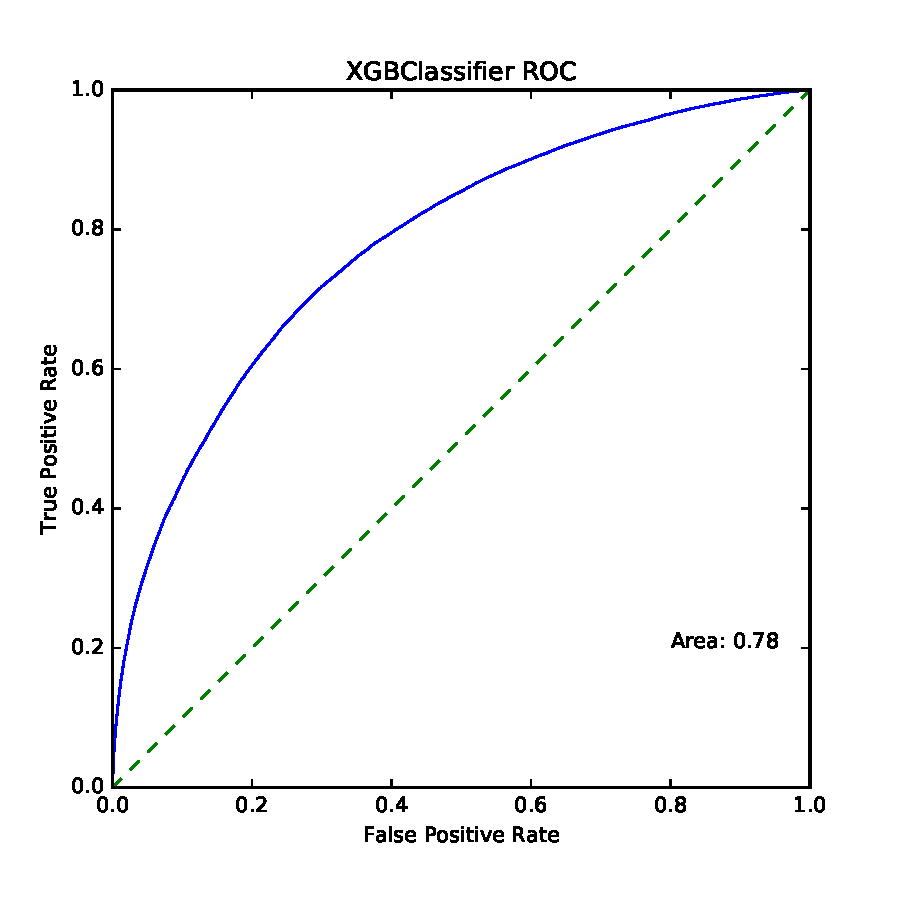
\includegraphics[width=0.8\columnwidth]{roc_curve_lowlevel.pdf}
%   \caption{ROC curve from XGBoost output. The classifier is trained only using the 21 low level inputs.}
% \end{figure}

% \paragraph{}
To explore how much XGBoost has exploited the non-linear correlations among the features, the distribution of one of the constructed feature is shown versus the classifier output, for the two cases trained with and without constructed features. This comparison is shown in Figure ~\ref{fig:roc_curve_lowlevel}.
\begin{figure}[!h]
  \label{fig:roc_curve_lowlevel}
  \centering
  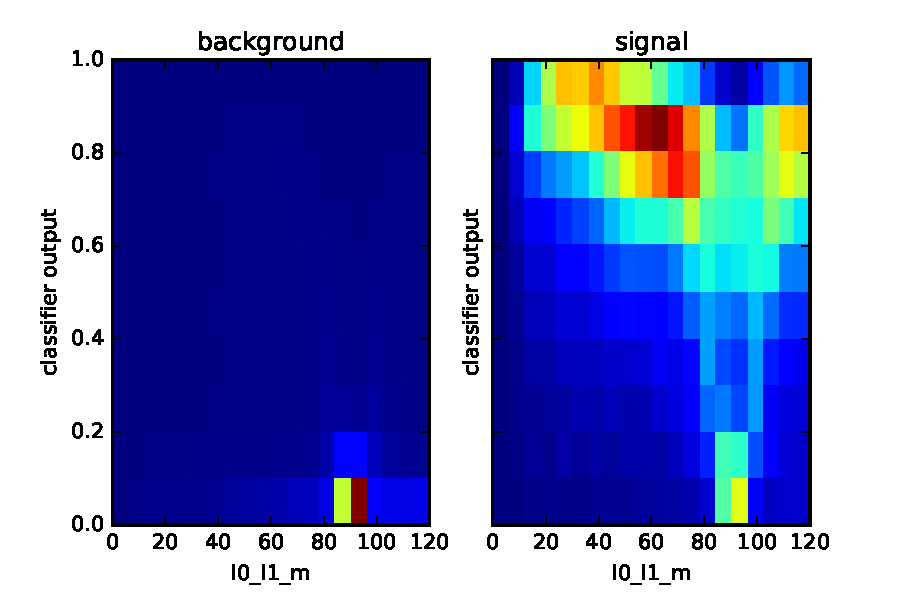
\includegraphics[width=\columnwidth]{l0_l1_m_highlevel.pdf}
  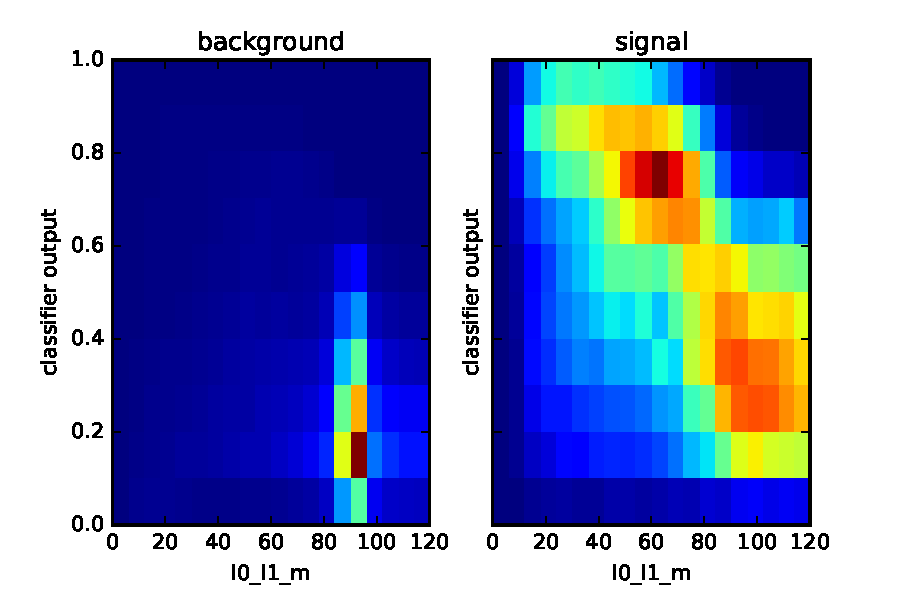
\includegraphics[width=\columnwidth]{l0_l1_m_lowlevel.pdf}
  \caption{Classifier output as a function of $l_0-l_1$ mass. On the x-axis one of the constructed feature is shown, whereas the y-axis refers to the output from the XGBoost classifier. The color-map shows to the number of events. The left column is for background, the right column is for signal. The top row is for the XGBoost classifier trained with all the features, while the bottom row is for the XGBoost classifier trained only with the simple features.}
\end{figure}
% \paragraph{}
The feature shown in the plot is the highest ranked variable in the full-feature-trained XGBoost classifier. The distribution shows a great separation power between signal and background. It is noteworthy that the classifier trained only with simple features produces an output which favors a similar region of space as the classifier trained with all the constructed features. In other words, the classifier exploited part but not all of the correlation in the low level input variables. This means that more work needs to be done in tuning the training parameters, and in further exploring the architectures for constructing better adaptive basis.

%%%%%%%%%%%%%%
\section{Conclusion}
%What happened?
%What next?
To summarize, this work has successfully shown the power of the application of machine learning techniques to the optimization of the signal region for a discovery of a new process in particle physics. The problem has been decomposed into two steps. First,  classification algorithms are used to distinguish signal and background. For this step, three different architecture has been tested: one-layer neural network, four-layers neural network, and XGBoost decision trees. Subsequently, the signal region has been built by interpreting the classifier output as the signal to background ratio for each point of the feature space, and by optimizing the selection on this variable.

The project has been tested on a synthetic dataset produced by the ATLAS experiment, related to the W$^{\pm}$W$^{\pm}$W$^{\mp}$ analysis. Features are either reconstructed particle characteristics, which are classified as \textit{simple} features, or higher level combination of the simple ones, on a basis of a physical motivation. The current methods from Neural Network or Boosted Decision Trees both outperform the previous baseline cut-based in terms of signal separation.
The optimization of the signal region definition allowed eventually to obtain a total significance 43\% larger than the baseline.
Additionally, a comparison between the architecture trained with only simple features, or with the addition of constructed features, has been performed. This analysis has shown that the adaptive basis is able to partially the correlation among the variables to reproduce the constructed variables, although only partially.

Some future directions of this work involve adding more background processes, and refining the network structure.

Specifically, at the moment only one major background is considered in the dataset, and since different physics processes generate different distribution of the features, it is expected that the current architectures, trained with only one background process, will not perform in the same way with more background. More detailed studies need to follow.

Moreover, one ultimate goal would be to build a software package that could take input as signal and backgrounds with raw input variables, and return a list of higher order \textbf{re-combined} variables that will distinguish the signal and background. 
The work which has been done in understanding the capabilities of the adaptive basis show that more effort is needed in order to tune properly the architecture and the training hyper-parameters.
This method could then be widely applied not only in high energy physics research, but in general on all kinds of real world problems. Due to the complexity, this goal may be hard to achieve by the end of this year but will worth continued exploration based on the result of this project.

% \section*{Acknowledgements}

% \textbf{Do not} include acknowledgements in the initial version of
% the paper submitted for blind review.

% If a paper is accepted, the final camera-ready version can (and
% probably should) include acknowledgements. In this case, please
% place such acknowledgements in an unnumbered section at the
% end of the paper. Typically, this will include thanks to reviewers
% who gave useful comments, to colleagues who contributed to the ideas,
% and to funding agencies and corporate sponsors that provided financial
% support.


\bibliography{example}
\bibliographystyle{icml2017}

\end{document}
